% Created by tikzDevice version 0.12.6 on 2024-03-09 10:51:46
% !TEX encoding = UTF-8 Unicode
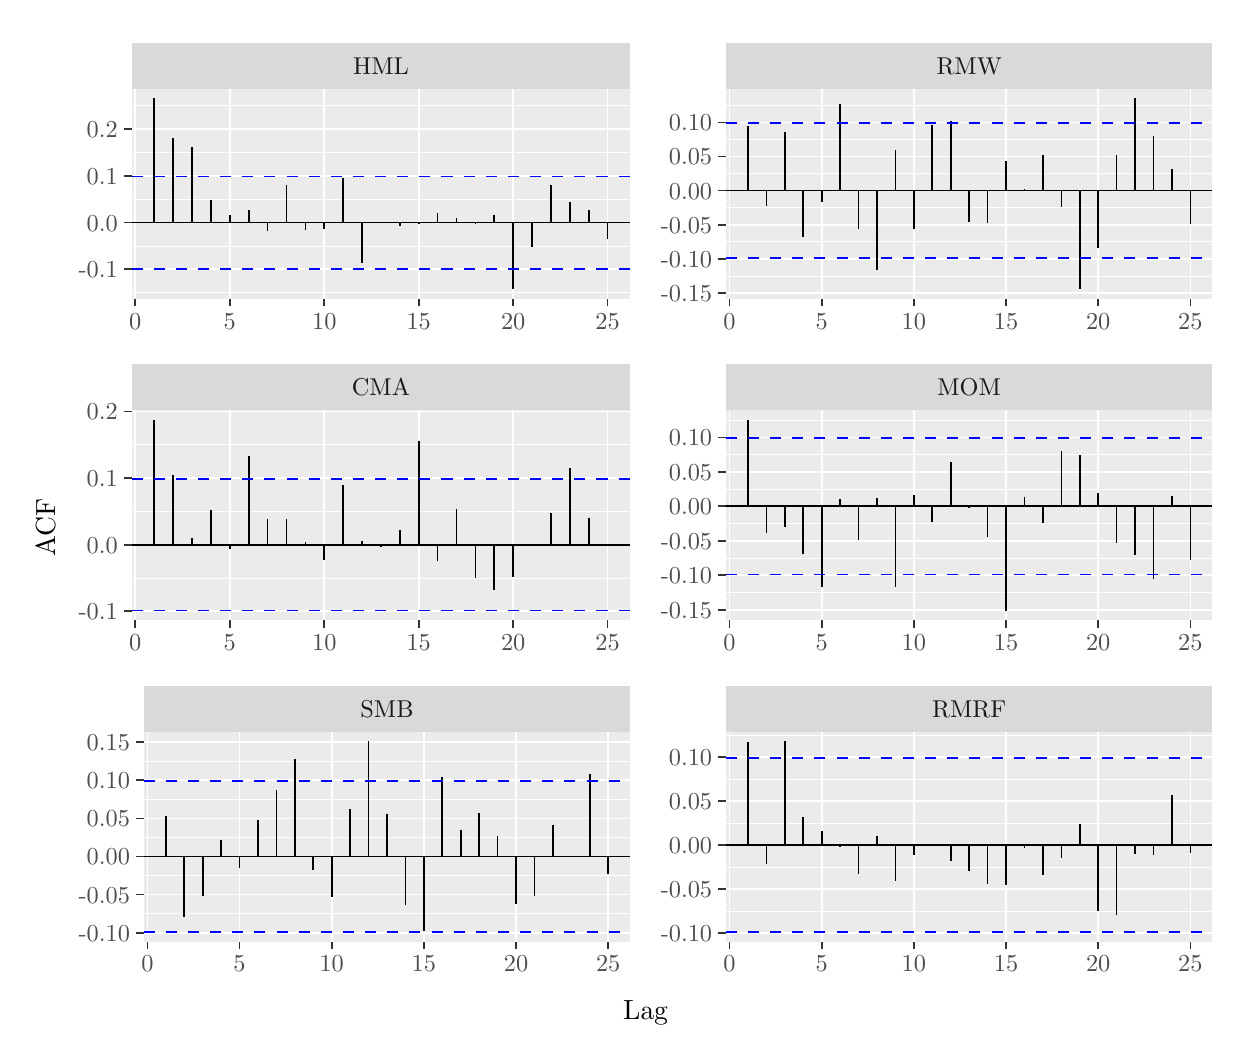
\begin{tikzpicture}[x=1pt,y=1pt]
\definecolor{fillColor}{RGB}{255,255,255}
\path[use as bounding box,fill=fillColor,fill opacity=0.00] (0,0) rectangle (433.62,361.35);
\begin{scope}
\path[clip] ( 12.91,245.20) rectangle (223.26,361.35);
\definecolor{drawColor}{RGB}{255,255,255}
\definecolor{fillColor}{RGB}{255,255,255}

\path[draw=drawColor,line width= 0.6pt,line join=round,line cap=round,fill=fillColor] ( 12.91,245.20) rectangle (223.26,361.35);
\end{scope}
\begin{scope}
\path[clip] ( 37.53,263.42) rectangle (217.76,339.28);
\definecolor{fillColor}{gray}{0.92}

\path[fill=fillColor] ( 37.53,263.42) rectangle (217.76,339.28);
\definecolor{drawColor}{RGB}{255,255,255}

\path[draw=drawColor,line width= 0.3pt,line join=round] ( 37.53,265.60) --
	(217.76,265.60);

\path[draw=drawColor,line width= 0.3pt,line join=round] ( 37.53,282.47) --
	(217.76,282.47);

\path[draw=drawColor,line width= 0.3pt,line join=round] ( 37.53,299.34) --
	(217.76,299.34);

\path[draw=drawColor,line width= 0.3pt,line join=round] ( 37.53,316.21) --
	(217.76,316.21);

\path[draw=drawColor,line width= 0.3pt,line join=round] ( 37.53,333.08) --
	(217.76,333.08);

\path[draw=drawColor,line width= 0.6pt,line join=round] ( 37.53,274.03) --
	(217.76,274.03);

\path[draw=drawColor,line width= 0.6pt,line join=round] ( 37.53,290.90) --
	(217.76,290.90);

\path[draw=drawColor,line width= 0.6pt,line join=round] ( 37.53,307.77) --
	(217.76,307.77);

\path[draw=drawColor,line width= 0.6pt,line join=round] ( 37.53,324.64) --
	(217.76,324.64);

\path[draw=drawColor,line width= 0.6pt,line join=round] ( 38.90,263.42) --
	( 38.90,339.28);

\path[draw=drawColor,line width= 0.6pt,line join=round] ( 73.03,263.42) --
	( 73.03,339.28);

\path[draw=drawColor,line width= 0.6pt,line join=round] (107.17,263.42) --
	(107.17,339.28);

\path[draw=drawColor,line width= 0.6pt,line join=round] (141.30,263.42) --
	(141.30,339.28);

\path[draw=drawColor,line width= 0.6pt,line join=round] (175.44,263.42) --
	(175.44,339.28);

\path[draw=drawColor,line width= 0.6pt,line join=round] (209.57,263.42) --
	(209.57,339.28);
\definecolor{drawColor}{RGB}{0,0,0}

\path[draw=drawColor,line width= 0.6pt,line join=round] ( 37.53,290.90) -- (217.76,290.90);

\path[draw=drawColor,line width= 0.6pt,line join=round] ( 45.73,290.90) -- ( 45.73,335.83);

\path[draw=drawColor,line width= 0.6pt,line join=round] ( 52.55,290.90) -- ( 52.55,321.49);

\path[draw=drawColor,line width= 0.6pt,line join=round] ( 59.38,290.90) -- ( 59.38,318.10);

\path[draw=drawColor,line width= 0.6pt,line join=round] ( 66.21,290.90) -- ( 66.21,299.08);

\path[draw=drawColor,line width= 0.6pt,line join=round] ( 73.03,290.90) -- ( 73.03,293.55);

\path[draw=drawColor,line width= 0.6pt,line join=round] ( 79.86,290.90) -- ( 79.86,295.48);

\path[draw=drawColor,line width= 0.6pt,line join=round] ( 86.69,290.90) -- ( 86.69,287.70);

\path[draw=drawColor,line width= 0.6pt,line join=round] ( 93.51,290.90) -- ( 93.51,304.48);

\path[draw=drawColor,line width= 0.6pt,line join=round] (100.34,290.90) -- (100.34,288.06);

\path[draw=drawColor,line width= 0.6pt,line join=round] (107.17,290.90) -- (107.17,288.60);

\path[draw=drawColor,line width= 0.6pt,line join=round] (114.00,290.90) -- (114.00,307.12);

\path[draw=drawColor,line width= 0.6pt,line join=round] (120.82,290.90) -- (120.82,276.32);

\path[draw=drawColor,line width= 0.6pt,line join=round] (127.65,290.90) -- (127.65,291.24);

\path[draw=drawColor,line width= 0.6pt,line join=round] (134.48,290.90) -- (134.48,289.66);

\path[draw=drawColor,line width= 0.6pt,line join=round] (141.30,290.90) -- (141.30,290.23);

\path[draw=drawColor,line width= 0.6pt,line join=round] (148.13,290.90) -- (148.13,294.36);

\path[draw=drawColor,line width= 0.6pt,line join=round] (154.96,290.90) -- (154.96,292.53);

\path[draw=drawColor,line width= 0.6pt,line join=round] (161.78,290.90) -- (161.78,290.23);

\path[draw=drawColor,line width= 0.6pt,line join=round] (168.61,290.90) -- (168.61,293.65);

\path[draw=drawColor,line width= 0.6pt,line join=round] (175.44,290.90) -- (175.44,266.87);

\path[draw=drawColor,line width= 0.6pt,line join=round] (182.26,290.90) -- (182.26,281.99);

\path[draw=drawColor,line width= 0.6pt,line join=round] (189.09,290.90) -- (189.09,304.52);

\path[draw=drawColor,line width= 0.6pt,line join=round] (195.92,290.90) -- (195.92,298.22);

\path[draw=drawColor,line width= 0.6pt,line join=round] (202.75,290.90) -- (202.75,295.41);

\path[draw=drawColor,line width= 0.6pt,line join=round] (209.57,290.90) -- (209.57,284.82);
\definecolor{drawColor}{RGB}{0,0,255}

\path[draw=drawColor,line width= 0.6pt,dash pattern=on 4pt off 4pt ,line join=round] ( 37.53,274.22) -- (217.76,274.22);

\path[draw=drawColor,line width= 0.6pt,dash pattern=on 4pt off 4pt ,line join=round] ( 37.53,307.58) -- (217.76,307.58);
\end{scope}
\begin{scope}
\path[clip] ( 37.53,339.28) rectangle (217.76,355.85);
\definecolor{fillColor}{gray}{0.85}

\path[fill=fillColor] ( 37.53,339.28) rectangle (217.76,355.85);
\definecolor{drawColor}{gray}{0.10}

\node[text=drawColor,anchor=base,inner sep=0pt, outer sep=0pt, scale=  0.88] at (127.65,344.53) {HML};
\end{scope}
\begin{scope}
\path[clip] (  0.00,  0.00) rectangle (433.62,361.35);
\definecolor{drawColor}{gray}{0.20}

\path[draw=drawColor,line width= 0.6pt,line join=round] ( 38.90,260.67) --
	( 38.90,263.42);

\path[draw=drawColor,line width= 0.6pt,line join=round] ( 73.03,260.67) --
	( 73.03,263.42);

\path[draw=drawColor,line width= 0.6pt,line join=round] (107.17,260.67) --
	(107.17,263.42);

\path[draw=drawColor,line width= 0.6pt,line join=round] (141.30,260.67) --
	(141.30,263.42);

\path[draw=drawColor,line width= 0.6pt,line join=round] (175.44,260.67) --
	(175.44,263.42);

\path[draw=drawColor,line width= 0.6pt,line join=round] (209.57,260.67) --
	(209.57,263.42);
\end{scope}
\begin{scope}
\path[clip] (  0.00,  0.00) rectangle (433.62,361.35);
\definecolor{drawColor}{gray}{0.30}

\node[text=drawColor,anchor=base,inner sep=0pt, outer sep=0pt, scale=  0.88] at ( 38.90,252.41) {0};

\node[text=drawColor,anchor=base,inner sep=0pt, outer sep=0pt, scale=  0.88] at ( 73.03,252.41) {5};

\node[text=drawColor,anchor=base,inner sep=0pt, outer sep=0pt, scale=  0.88] at (107.17,252.41) {10};

\node[text=drawColor,anchor=base,inner sep=0pt, outer sep=0pt, scale=  0.88] at (141.30,252.41) {15};

\node[text=drawColor,anchor=base,inner sep=0pt, outer sep=0pt, scale=  0.88] at (175.44,252.41) {20};

\node[text=drawColor,anchor=base,inner sep=0pt, outer sep=0pt, scale=  0.88] at (209.57,252.41) {25};
\end{scope}
\begin{scope}
\path[clip] (  0.00,  0.00) rectangle (433.62,361.35);
\definecolor{drawColor}{gray}{0.30}

\node[text=drawColor,anchor=base east,inner sep=0pt, outer sep=0pt, scale=  0.88] at ( 32.58,271.00) {-0.1};

\node[text=drawColor,anchor=base east,inner sep=0pt, outer sep=0pt, scale=  0.88] at ( 32.58,287.87) {0.0};

\node[text=drawColor,anchor=base east,inner sep=0pt, outer sep=0pt, scale=  0.88] at ( 32.58,304.74) {0.1};

\node[text=drawColor,anchor=base east,inner sep=0pt, outer sep=0pt, scale=  0.88] at ( 32.58,321.61) {0.2};
\end{scope}
\begin{scope}
\path[clip] (  0.00,  0.00) rectangle (433.62,361.35);
\definecolor{drawColor}{gray}{0.20}

\path[draw=drawColor,line width= 0.6pt,line join=round] ( 34.78,274.03) --
	( 37.53,274.03);

\path[draw=drawColor,line width= 0.6pt,line join=round] ( 34.78,290.90) --
	( 37.53,290.90);

\path[draw=drawColor,line width= 0.6pt,line join=round] ( 34.78,307.77) --
	( 37.53,307.77);

\path[draw=drawColor,line width= 0.6pt,line join=round] ( 34.78,324.64) --
	( 37.53,324.64);
\end{scope}
\begin{scope}
\path[clip] (223.26,245.20) rectangle (433.62,361.35);
\definecolor{drawColor}{RGB}{255,255,255}
\definecolor{fillColor}{RGB}{255,255,255}

\path[draw=drawColor,line width= 0.6pt,line join=round,line cap=round,fill=fillColor] (223.26,245.20) rectangle (433.62,361.35);
\end{scope}
\begin{scope}
\path[clip] (252.29,263.42) rectangle (428.12,339.28);
\definecolor{fillColor}{gray}{0.92}

\path[fill=fillColor] (252.29,263.42) rectangle (428.12,339.28);
\definecolor{drawColor}{RGB}{255,255,255}

\path[draw=drawColor,line width= 0.3pt,line join=round] (252.29,271.64) --
	(428.12,271.64);

\path[draw=drawColor,line width= 0.3pt,line join=round] (252.29,283.97) --
	(428.12,283.97);

\path[draw=drawColor,line width= 0.3pt,line join=round] (252.29,296.29) --
	(428.12,296.29);

\path[draw=drawColor,line width= 0.3pt,line join=round] (252.29,308.62) --
	(428.12,308.62);

\path[draw=drawColor,line width= 0.3pt,line join=round] (252.29,320.94) --
	(428.12,320.94);

\path[draw=drawColor,line width= 0.3pt,line join=round] (252.29,333.27) --
	(428.12,333.27);

\path[draw=drawColor,line width= 0.6pt,line join=round] (252.29,265.48) --
	(428.12,265.48);

\path[draw=drawColor,line width= 0.6pt,line join=round] (252.29,277.80) --
	(428.12,277.80);

\path[draw=drawColor,line width= 0.6pt,line join=round] (252.29,290.13) --
	(428.12,290.13);

\path[draw=drawColor,line width= 0.6pt,line join=round] (252.29,302.46) --
	(428.12,302.46);

\path[draw=drawColor,line width= 0.6pt,line join=round] (252.29,314.78) --
	(428.12,314.78);

\path[draw=drawColor,line width= 0.6pt,line join=round] (252.29,327.11) --
	(428.12,327.11);

\path[draw=drawColor,line width= 0.6pt,line join=round] (253.62,263.42) --
	(253.62,339.28);

\path[draw=drawColor,line width= 0.6pt,line join=round] (286.92,263.42) --
	(286.92,339.28);

\path[draw=drawColor,line width= 0.6pt,line join=round] (320.22,263.42) --
	(320.22,339.28);

\path[draw=drawColor,line width= 0.6pt,line join=round] (353.52,263.42) --
	(353.52,339.28);

\path[draw=drawColor,line width= 0.6pt,line join=round] (386.83,263.42) --
	(386.83,339.28);

\path[draw=drawColor,line width= 0.6pt,line join=round] (420.13,263.42) --
	(420.13,339.28);
\definecolor{drawColor}{RGB}{0,0,0}

\path[draw=drawColor,line width= 0.6pt,line join=round] (252.29,302.46) -- (428.12,302.46);

\path[draw=drawColor,line width= 0.6pt,line join=round] (260.28,302.46) -- (260.28,325.99);

\path[draw=drawColor,line width= 0.6pt,line join=round] (266.94,302.46) -- (266.94,296.86);

\path[draw=drawColor,line width= 0.6pt,line join=round] (273.60,302.46) -- (273.60,323.74);

\path[draw=drawColor,line width= 0.6pt,line join=round] (280.26,302.46) -- (280.26,285.78);

\path[draw=drawColor,line width= 0.6pt,line join=round] (286.92,302.46) -- (286.92,298.36);

\path[draw=drawColor,line width= 0.6pt,line join=round] (293.58,302.46) -- (293.58,333.59);

\path[draw=drawColor,line width= 0.6pt,line join=round] (300.24,302.46) -- (300.24,288.76);

\path[draw=drawColor,line width= 0.6pt,line join=round] (306.90,302.46) -- (306.90,273.76);

\path[draw=drawColor,line width= 0.6pt,line join=round] (313.56,302.46) -- (313.56,317.10);

\path[draw=drawColor,line width= 0.6pt,line join=round] (320.22,302.46) -- (320.22,288.64);

\path[draw=drawColor,line width= 0.6pt,line join=round] (326.88,302.46) -- (326.88,326.00);

\path[draw=drawColor,line width= 0.6pt,line join=round] (333.54,302.46) -- (333.54,327.77);

\path[draw=drawColor,line width= 0.6pt,line join=round] (340.20,302.46) -- (340.20,291.11);

\path[draw=drawColor,line width= 0.6pt,line join=round] (346.86,302.46) -- (346.86,290.89);

\path[draw=drawColor,line width= 0.6pt,line join=round] (353.52,302.46) -- (353.52,313.15);

\path[draw=drawColor,line width= 0.6pt,line join=round] (360.18,302.46) -- (360.18,303.15);

\path[draw=drawColor,line width= 0.6pt,line join=round] (366.85,302.46) -- (366.85,315.32);

\path[draw=drawColor,line width= 0.6pt,line join=round] (373.51,302.46) -- (373.51,296.53);

\path[draw=drawColor,line width= 0.6pt,line join=round] (380.17,302.46) -- (380.17,266.87);

\path[draw=drawColor,line width= 0.6pt,line join=round] (386.83,302.46) -- (386.83,281.58);

\path[draw=drawColor,line width= 0.6pt,line join=round] (393.49,302.46) -- (393.49,315.46);

\path[draw=drawColor,line width= 0.6pt,line join=round] (400.15,302.46) -- (400.15,335.83);

\path[draw=drawColor,line width= 0.6pt,line join=round] (406.81,302.46) -- (406.81,322.16);

\path[draw=drawColor,line width= 0.6pt,line join=round] (413.47,302.46) -- (413.47,310.37);

\path[draw=drawColor,line width= 0.6pt,line join=round] (420.13,302.46) -- (420.13,290.56);
\definecolor{drawColor}{RGB}{0,0,255}

\path[draw=drawColor,line width= 0.6pt,dash pattern=on 4pt off 4pt ,line join=round] (252.29,278.08) -- (428.12,278.08);

\path[draw=drawColor,line width= 0.6pt,dash pattern=on 4pt off 4pt ,line join=round] (252.29,326.83) -- (428.12,326.83);
\end{scope}
\begin{scope}
\path[clip] (252.29,339.28) rectangle (428.12,355.85);
\definecolor{fillColor}{gray}{0.85}

\path[fill=fillColor] (252.29,339.28) rectangle (428.12,355.85);
\definecolor{drawColor}{gray}{0.10}

\node[text=drawColor,anchor=base,inner sep=0pt, outer sep=0pt, scale=  0.88] at (340.20,344.53) {RMW};
\end{scope}
\begin{scope}
\path[clip] (  0.00,  0.00) rectangle (433.62,361.35);
\definecolor{drawColor}{gray}{0.20}

\path[draw=drawColor,line width= 0.6pt,line join=round] (253.62,260.67) --
	(253.62,263.42);

\path[draw=drawColor,line width= 0.6pt,line join=round] (286.92,260.67) --
	(286.92,263.42);

\path[draw=drawColor,line width= 0.6pt,line join=round] (320.22,260.67) --
	(320.22,263.42);

\path[draw=drawColor,line width= 0.6pt,line join=round] (353.52,260.67) --
	(353.52,263.42);

\path[draw=drawColor,line width= 0.6pt,line join=round] (386.83,260.67) --
	(386.83,263.42);

\path[draw=drawColor,line width= 0.6pt,line join=round] (420.13,260.67) --
	(420.13,263.42);
\end{scope}
\begin{scope}
\path[clip] (  0.00,  0.00) rectangle (433.62,361.35);
\definecolor{drawColor}{gray}{0.30}

\node[text=drawColor,anchor=base,inner sep=0pt, outer sep=0pt, scale=  0.88] at (253.62,252.41) {0};

\node[text=drawColor,anchor=base,inner sep=0pt, outer sep=0pt, scale=  0.88] at (286.92,252.41) {5};

\node[text=drawColor,anchor=base,inner sep=0pt, outer sep=0pt, scale=  0.88] at (320.22,252.41) {10};

\node[text=drawColor,anchor=base,inner sep=0pt, outer sep=0pt, scale=  0.88] at (353.52,252.41) {15};

\node[text=drawColor,anchor=base,inner sep=0pt, outer sep=0pt, scale=  0.88] at (386.83,252.41) {20};

\node[text=drawColor,anchor=base,inner sep=0pt, outer sep=0pt, scale=  0.88] at (420.13,252.41) {25};
\end{scope}
\begin{scope}
\path[clip] (  0.00,  0.00) rectangle (433.62,361.35);
\definecolor{drawColor}{gray}{0.30}

\node[text=drawColor,anchor=base east,inner sep=0pt, outer sep=0pt, scale=  0.88] at (247.34,262.45) {-0.15};

\node[text=drawColor,anchor=base east,inner sep=0pt, outer sep=0pt, scale=  0.88] at (247.34,274.77) {-0.10};

\node[text=drawColor,anchor=base east,inner sep=0pt, outer sep=0pt, scale=  0.88] at (247.34,287.10) {-0.05};

\node[text=drawColor,anchor=base east,inner sep=0pt, outer sep=0pt, scale=  0.88] at (247.34,299.42) {0.00};

\node[text=drawColor,anchor=base east,inner sep=0pt, outer sep=0pt, scale=  0.88] at (247.34,311.75) {0.05};

\node[text=drawColor,anchor=base east,inner sep=0pt, outer sep=0pt, scale=  0.88] at (247.34,324.08) {0.10};
\end{scope}
\begin{scope}
\path[clip] (  0.00,  0.00) rectangle (433.62,361.35);
\definecolor{drawColor}{gray}{0.20}

\path[draw=drawColor,line width= 0.6pt,line join=round] (249.54,265.48) --
	(252.29,265.48);

\path[draw=drawColor,line width= 0.6pt,line join=round] (249.54,277.80) --
	(252.29,277.80);

\path[draw=drawColor,line width= 0.6pt,line join=round] (249.54,290.13) --
	(252.29,290.13);

\path[draw=drawColor,line width= 0.6pt,line join=round] (249.54,302.46) --
	(252.29,302.46);

\path[draw=drawColor,line width= 0.6pt,line join=round] (249.54,314.78) --
	(252.29,314.78);

\path[draw=drawColor,line width= 0.6pt,line join=round] (249.54,327.11) --
	(252.29,327.11);
\end{scope}
\begin{scope}
\path[clip] ( 12.91,129.06) rectangle (223.26,245.20);
\definecolor{drawColor}{RGB}{255,255,255}
\definecolor{fillColor}{RGB}{255,255,255}

\path[draw=drawColor,line width= 0.6pt,line join=round,line cap=round,fill=fillColor] ( 12.91,129.06) rectangle (223.26,245.20);
\end{scope}
\begin{scope}
\path[clip] ( 37.53,147.28) rectangle (217.76,223.13);
\definecolor{fillColor}{gray}{0.92}

\path[fill=fillColor] ( 37.53,147.28) rectangle (217.76,223.13);
\definecolor{drawColor}{RGB}{255,255,255}

\path[draw=drawColor,line width= 0.3pt,line join=round] ( 37.53,162.49) --
	(217.76,162.49);

\path[draw=drawColor,line width= 0.3pt,line join=round] ( 37.53,186.57) --
	(217.76,186.57);

\path[draw=drawColor,line width= 0.3pt,line join=round] ( 37.53,210.65) --
	(217.76,210.65);

\path[draw=drawColor,line width= 0.6pt,line join=round] ( 37.53,150.45) --
	(217.76,150.45);

\path[draw=drawColor,line width= 0.6pt,line join=round] ( 37.53,174.53) --
	(217.76,174.53);

\path[draw=drawColor,line width= 0.6pt,line join=round] ( 37.53,198.61) --
	(217.76,198.61);

\path[draw=drawColor,line width= 0.6pt,line join=round] ( 37.53,222.68) --
	(217.76,222.68);

\path[draw=drawColor,line width= 0.6pt,line join=round] ( 38.90,147.28) --
	( 38.90,223.13);

\path[draw=drawColor,line width= 0.6pt,line join=round] ( 73.03,147.28) --
	( 73.03,223.13);

\path[draw=drawColor,line width= 0.6pt,line join=round] (107.17,147.28) --
	(107.17,223.13);

\path[draw=drawColor,line width= 0.6pt,line join=round] (141.30,147.28) --
	(141.30,223.13);

\path[draw=drawColor,line width= 0.6pt,line join=round] (175.44,147.28) --
	(175.44,223.13);

\path[draw=drawColor,line width= 0.6pt,line join=round] (209.57,147.28) --
	(209.57,223.13);
\definecolor{drawColor}{RGB}{0,0,0}

\path[draw=drawColor,line width= 0.6pt,line join=round] ( 37.53,174.53) -- (217.76,174.53);

\path[draw=drawColor,line width= 0.6pt,line join=round] ( 45.73,174.53) -- ( 45.73,219.68);

\path[draw=drawColor,line width= 0.6pt,line join=round] ( 52.55,174.53) -- ( 52.55,199.77);

\path[draw=drawColor,line width= 0.6pt,line join=round] ( 59.38,174.53) -- ( 59.38,177.12);

\path[draw=drawColor,line width= 0.6pt,line join=round] ( 66.21,174.53) -- ( 66.21,187.08);

\path[draw=drawColor,line width= 0.6pt,line join=round] ( 73.03,174.53) -- ( 73.03,173.10);

\path[draw=drawColor,line width= 0.6pt,line join=round] ( 79.86,174.53) -- ( 79.86,206.74);

\path[draw=drawColor,line width= 0.6pt,line join=round] ( 86.69,174.53) -- ( 86.69,183.67);

\path[draw=drawColor,line width= 0.6pt,line join=round] ( 93.51,174.53) -- ( 93.51,183.64);

\path[draw=drawColor,line width= 0.6pt,line join=round] (100.34,174.53) -- (100.34,175.46);

\path[draw=drawColor,line width= 0.6pt,line join=round] (107.17,174.53) -- (107.17,168.87);

\path[draw=drawColor,line width= 0.6pt,line join=round] (114.00,174.53) -- (114.00,196.01);

\path[draw=drawColor,line width= 0.6pt,line join=round] (120.82,174.53) -- (120.82,175.73);

\path[draw=drawColor,line width= 0.6pt,line join=round] (127.65,174.53) -- (127.65,173.69);

\path[draw=drawColor,line width= 0.6pt,line join=round] (134.48,174.53) -- (134.48,179.90);

\path[draw=drawColor,line width= 0.6pt,line join=round] (141.30,174.53) -- (141.30,211.86);

\path[draw=drawColor,line width= 0.6pt,line join=round] (148.13,174.53) -- (148.13,168.52);

\path[draw=drawColor,line width= 0.6pt,line join=round] (154.96,174.53) -- (154.96,187.31);

\path[draw=drawColor,line width= 0.6pt,line join=round] (161.78,174.53) -- (161.78,162.62);

\path[draw=drawColor,line width= 0.6pt,line join=round] (168.61,174.53) -- (168.61,158.12);

\path[draw=drawColor,line width= 0.6pt,line join=round] (175.44,174.53) -- (175.44,162.93);

\path[draw=drawColor,line width= 0.6pt,line join=round] (182.26,174.53) -- (182.26,174.25);

\path[draw=drawColor,line width= 0.6pt,line join=round] (189.09,174.53) -- (189.09,185.98);

\path[draw=drawColor,line width= 0.6pt,line join=round] (195.92,174.53) -- (195.92,202.32);

\path[draw=drawColor,line width= 0.6pt,line join=round] (202.75,174.53) -- (202.75,184.23);

\path[draw=drawColor,line width= 0.6pt,line join=round] (209.57,174.53) -- (209.57,174.24);
\definecolor{drawColor}{RGB}{0,0,255}

\path[draw=drawColor,line width= 0.6pt,dash pattern=on 4pt off 4pt ,line join=round] ( 37.53,150.73) -- (217.76,150.73);

\path[draw=drawColor,line width= 0.6pt,dash pattern=on 4pt off 4pt ,line join=round] ( 37.53,198.33) -- (217.76,198.33);
\end{scope}
\begin{scope}
\path[clip] ( 37.53,223.13) rectangle (217.76,239.70);
\definecolor{fillColor}{gray}{0.85}

\path[fill=fillColor] ( 37.53,223.13) rectangle (217.76,239.70);
\definecolor{drawColor}{gray}{0.10}

\node[text=drawColor,anchor=base,inner sep=0pt, outer sep=0pt, scale=  0.88] at (127.65,228.39) {CMA};
\end{scope}
\begin{scope}
\path[clip] (  0.00,  0.00) rectangle (433.62,361.35);
\definecolor{drawColor}{gray}{0.20}

\path[draw=drawColor,line width= 0.6pt,line join=round] ( 38.90,144.53) --
	( 38.90,147.28);

\path[draw=drawColor,line width= 0.6pt,line join=round] ( 73.03,144.53) --
	( 73.03,147.28);

\path[draw=drawColor,line width= 0.6pt,line join=round] (107.17,144.53) --
	(107.17,147.28);

\path[draw=drawColor,line width= 0.6pt,line join=round] (141.30,144.53) --
	(141.30,147.28);

\path[draw=drawColor,line width= 0.6pt,line join=round] (175.44,144.53) --
	(175.44,147.28);

\path[draw=drawColor,line width= 0.6pt,line join=round] (209.57,144.53) --
	(209.57,147.28);
\end{scope}
\begin{scope}
\path[clip] (  0.00,  0.00) rectangle (433.62,361.35);
\definecolor{drawColor}{gray}{0.30}

\node[text=drawColor,anchor=base,inner sep=0pt, outer sep=0pt, scale=  0.88] at ( 38.90,136.27) {0};

\node[text=drawColor,anchor=base,inner sep=0pt, outer sep=0pt, scale=  0.88] at ( 73.03,136.27) {5};

\node[text=drawColor,anchor=base,inner sep=0pt, outer sep=0pt, scale=  0.88] at (107.17,136.27) {10};

\node[text=drawColor,anchor=base,inner sep=0pt, outer sep=0pt, scale=  0.88] at (141.30,136.27) {15};

\node[text=drawColor,anchor=base,inner sep=0pt, outer sep=0pt, scale=  0.88] at (175.44,136.27) {20};

\node[text=drawColor,anchor=base,inner sep=0pt, outer sep=0pt, scale=  0.88] at (209.57,136.27) {25};
\end{scope}
\begin{scope}
\path[clip] (  0.00,  0.00) rectangle (433.62,361.35);
\definecolor{drawColor}{gray}{0.30}

\node[text=drawColor,anchor=base east,inner sep=0pt, outer sep=0pt, scale=  0.88] at ( 32.58,147.42) {-0.1};

\node[text=drawColor,anchor=base east,inner sep=0pt, outer sep=0pt, scale=  0.88] at ( 32.58,171.50) {0.0};

\node[text=drawColor,anchor=base east,inner sep=0pt, outer sep=0pt, scale=  0.88] at ( 32.58,195.58) {0.1};

\node[text=drawColor,anchor=base east,inner sep=0pt, outer sep=0pt, scale=  0.88] at ( 32.58,219.65) {0.2};
\end{scope}
\begin{scope}
\path[clip] (  0.00,  0.00) rectangle (433.62,361.35);
\definecolor{drawColor}{gray}{0.20}

\path[draw=drawColor,line width= 0.6pt,line join=round] ( 34.78,150.45) --
	( 37.53,150.45);

\path[draw=drawColor,line width= 0.6pt,line join=round] ( 34.78,174.53) --
	( 37.53,174.53);

\path[draw=drawColor,line width= 0.6pt,line join=round] ( 34.78,198.61) --
	( 37.53,198.61);

\path[draw=drawColor,line width= 0.6pt,line join=round] ( 34.78,222.68) --
	( 37.53,222.68);
\end{scope}
\begin{scope}
\path[clip] (223.26,129.06) rectangle (433.62,245.20);
\definecolor{drawColor}{RGB}{255,255,255}
\definecolor{fillColor}{RGB}{255,255,255}

\path[draw=drawColor,line width= 0.6pt,line join=round,line cap=round,fill=fillColor] (223.26,129.06) rectangle (433.62,245.20);
\end{scope}
\begin{scope}
\path[clip] (252.29,147.28) rectangle (428.12,223.13);
\definecolor{fillColor}{gray}{0.92}

\path[fill=fillColor] (252.29,147.28) rectangle (428.12,223.13);
\definecolor{drawColor}{RGB}{255,255,255}

\path[draw=drawColor,line width= 0.3pt,line join=round] (252.29,157.27) --
	(428.12,157.27);

\path[draw=drawColor,line width= 0.3pt,line join=round] (252.29,169.72) --
	(428.12,169.72);

\path[draw=drawColor,line width= 0.3pt,line join=round] (252.29,182.17) --
	(428.12,182.17);

\path[draw=drawColor,line width= 0.3pt,line join=round] (252.29,194.62) --
	(428.12,194.62);

\path[draw=drawColor,line width= 0.3pt,line join=round] (252.29,207.07) --
	(428.12,207.07);

\path[draw=drawColor,line width= 0.3pt,line join=round] (252.29,219.52) --
	(428.12,219.52);

\path[draw=drawColor,line width= 0.6pt,line join=round] (252.29,151.04) --
	(428.12,151.04);

\path[draw=drawColor,line width= 0.6pt,line join=round] (252.29,163.49) --
	(428.12,163.49);

\path[draw=drawColor,line width= 0.6pt,line join=round] (252.29,175.94) --
	(428.12,175.94);

\path[draw=drawColor,line width= 0.6pt,line join=round] (252.29,188.39) --
	(428.12,188.39);

\path[draw=drawColor,line width= 0.6pt,line join=round] (252.29,200.84) --
	(428.12,200.84);

\path[draw=drawColor,line width= 0.6pt,line join=round] (252.29,213.29) --
	(428.12,213.29);

\path[draw=drawColor,line width= 0.6pt,line join=round] (253.62,147.28) --
	(253.62,223.13);

\path[draw=drawColor,line width= 0.6pt,line join=round] (286.92,147.28) --
	(286.92,223.13);

\path[draw=drawColor,line width= 0.6pt,line join=round] (320.22,147.28) --
	(320.22,223.13);

\path[draw=drawColor,line width= 0.6pt,line join=round] (353.52,147.28) --
	(353.52,223.13);

\path[draw=drawColor,line width= 0.6pt,line join=round] (386.83,147.28) --
	(386.83,223.13);

\path[draw=drawColor,line width= 0.6pt,line join=round] (420.13,147.28) --
	(420.13,223.13);
\definecolor{drawColor}{RGB}{0,0,0}

\path[draw=drawColor,line width= 0.6pt,line join=round] (252.29,188.39) -- (428.12,188.39);

\path[draw=drawColor,line width= 0.6pt,line join=round] (260.28,188.39) -- (260.28,219.68);

\path[draw=drawColor,line width= 0.6pt,line join=round] (266.94,188.39) -- (266.94,178.60);

\path[draw=drawColor,line width= 0.6pt,line join=round] (273.60,188.39) -- (273.60,180.99);

\path[draw=drawColor,line width= 0.6pt,line join=round] (280.26,188.39) -- (280.26,171.13);

\path[draw=drawColor,line width= 0.6pt,line join=round] (286.92,188.39) -- (286.92,159.34);

\path[draw=drawColor,line width= 0.6pt,line join=round] (293.58,188.39) -- (293.58,190.92);

\path[draw=drawColor,line width= 0.6pt,line join=round] (300.24,188.39) -- (300.24,176.08);

\path[draw=drawColor,line width= 0.6pt,line join=round] (306.90,188.39) -- (306.90,191.49);

\path[draw=drawColor,line width= 0.6pt,line join=round] (313.56,188.39) -- (313.56,159.09);

\path[draw=drawColor,line width= 0.6pt,line join=round] (320.22,188.39) -- (320.22,192.59);

\path[draw=drawColor,line width= 0.6pt,line join=round] (326.88,188.39) -- (326.88,182.69);

\path[draw=drawColor,line width= 0.6pt,line join=round] (333.54,188.39) -- (333.54,204.24);

\path[draw=drawColor,line width= 0.6pt,line join=round] (340.20,188.39) -- (340.20,187.74);

\path[draw=drawColor,line width= 0.6pt,line join=round] (346.86,188.39) -- (346.86,177.20);

\path[draw=drawColor,line width= 0.6pt,line join=round] (353.52,188.39) -- (353.52,150.73);

\path[draw=drawColor,line width= 0.6pt,line join=round] (360.18,188.39) -- (360.18,191.77);

\path[draw=drawColor,line width= 0.6pt,line join=round] (366.85,188.39) -- (366.85,182.29);

\path[draw=drawColor,line width= 0.6pt,line join=round] (373.51,188.39) -- (373.51,208.47);

\path[draw=drawColor,line width= 0.6pt,line join=round] (380.17,188.39) -- (380.17,206.82);

\path[draw=drawColor,line width= 0.6pt,line join=round] (386.83,188.39) -- (386.83,193.24);

\path[draw=drawColor,line width= 0.6pt,line join=round] (393.49,188.39) -- (393.49,175.18);

\path[draw=drawColor,line width= 0.6pt,line join=round] (400.15,188.39) -- (400.15,170.87);

\path[draw=drawColor,line width= 0.6pt,line join=round] (406.81,188.39) -- (406.81,162.02);

\path[draw=drawColor,line width= 0.6pt,line join=round] (413.47,188.39) -- (413.47,192.15);

\path[draw=drawColor,line width= 0.6pt,line join=round] (420.13,188.39) -- (420.13,168.93);
\definecolor{drawColor}{RGB}{0,0,255}

\path[draw=drawColor,line width= 0.6pt,dash pattern=on 4pt off 4pt ,line join=round] (252.29,163.77) -- (428.12,163.77);

\path[draw=drawColor,line width= 0.6pt,dash pattern=on 4pt off 4pt ,line join=round] (252.29,213.01) -- (428.12,213.01);
\end{scope}
\begin{scope}
\path[clip] (252.29,223.13) rectangle (428.12,239.70);
\definecolor{fillColor}{gray}{0.85}

\path[fill=fillColor] (252.29,223.13) rectangle (428.12,239.70);
\definecolor{drawColor}{gray}{0.10}

\node[text=drawColor,anchor=base,inner sep=0pt, outer sep=0pt, scale=  0.88] at (340.20,228.39) {MOM};
\end{scope}
\begin{scope}
\path[clip] (  0.00,  0.00) rectangle (433.62,361.35);
\definecolor{drawColor}{gray}{0.20}

\path[draw=drawColor,line width= 0.6pt,line join=round] (253.62,144.53) --
	(253.62,147.28);

\path[draw=drawColor,line width= 0.6pt,line join=round] (286.92,144.53) --
	(286.92,147.28);

\path[draw=drawColor,line width= 0.6pt,line join=round] (320.22,144.53) --
	(320.22,147.28);

\path[draw=drawColor,line width= 0.6pt,line join=round] (353.52,144.53) --
	(353.52,147.28);

\path[draw=drawColor,line width= 0.6pt,line join=round] (386.83,144.53) --
	(386.83,147.28);

\path[draw=drawColor,line width= 0.6pt,line join=round] (420.13,144.53) --
	(420.13,147.28);
\end{scope}
\begin{scope}
\path[clip] (  0.00,  0.00) rectangle (433.62,361.35);
\definecolor{drawColor}{gray}{0.30}

\node[text=drawColor,anchor=base,inner sep=0pt, outer sep=0pt, scale=  0.88] at (253.62,136.27) {0};

\node[text=drawColor,anchor=base,inner sep=0pt, outer sep=0pt, scale=  0.88] at (286.92,136.27) {5};

\node[text=drawColor,anchor=base,inner sep=0pt, outer sep=0pt, scale=  0.88] at (320.22,136.27) {10};

\node[text=drawColor,anchor=base,inner sep=0pt, outer sep=0pt, scale=  0.88] at (353.52,136.27) {15};

\node[text=drawColor,anchor=base,inner sep=0pt, outer sep=0pt, scale=  0.88] at (386.83,136.27) {20};

\node[text=drawColor,anchor=base,inner sep=0pt, outer sep=0pt, scale=  0.88] at (420.13,136.27) {25};
\end{scope}
\begin{scope}
\path[clip] (  0.00,  0.00) rectangle (433.62,361.35);
\definecolor{drawColor}{gray}{0.30}

\node[text=drawColor,anchor=base east,inner sep=0pt, outer sep=0pt, scale=  0.88] at (247.34,148.01) {-0.15};

\node[text=drawColor,anchor=base east,inner sep=0pt, outer sep=0pt, scale=  0.88] at (247.34,160.46) {-0.10};

\node[text=drawColor,anchor=base east,inner sep=0pt, outer sep=0pt, scale=  0.88] at (247.34,172.91) {-0.05};

\node[text=drawColor,anchor=base east,inner sep=0pt, outer sep=0pt, scale=  0.88] at (247.34,185.36) {0.00};

\node[text=drawColor,anchor=base east,inner sep=0pt, outer sep=0pt, scale=  0.88] at (247.34,197.81) {0.05};

\node[text=drawColor,anchor=base east,inner sep=0pt, outer sep=0pt, scale=  0.88] at (247.34,210.26) {0.10};
\end{scope}
\begin{scope}
\path[clip] (  0.00,  0.00) rectangle (433.62,361.35);
\definecolor{drawColor}{gray}{0.20}

\path[draw=drawColor,line width= 0.6pt,line join=round] (249.54,151.04) --
	(252.29,151.04);

\path[draw=drawColor,line width= 0.6pt,line join=round] (249.54,163.49) --
	(252.29,163.49);

\path[draw=drawColor,line width= 0.6pt,line join=round] (249.54,175.94) --
	(252.29,175.94);

\path[draw=drawColor,line width= 0.6pt,line join=round] (249.54,188.39) --
	(252.29,188.39);

\path[draw=drawColor,line width= 0.6pt,line join=round] (249.54,200.84) --
	(252.29,200.84);

\path[draw=drawColor,line width= 0.6pt,line join=round] (249.54,213.29) --
	(252.29,213.29);
\end{scope}
\begin{scope}
\path[clip] ( 12.91, 12.91) rectangle (223.26,129.06);
\definecolor{drawColor}{RGB}{255,255,255}
\definecolor{fillColor}{RGB}{255,255,255}

\path[draw=drawColor,line width= 0.6pt,line join=round,line cap=round,fill=fillColor] ( 12.91, 12.91) rectangle (223.26,129.06);
\end{scope}
\begin{scope}
\path[clip] ( 41.93, 31.13) rectangle (217.76,106.98);
\definecolor{fillColor}{gray}{0.92}

\path[fill=fillColor] ( 41.93, 31.13) rectangle (217.76,106.98);
\definecolor{drawColor}{RGB}{255,255,255}

\path[draw=drawColor,line width= 0.3pt,line join=round] ( 41.93, 41.16) --
	(217.76, 41.16);

\path[draw=drawColor,line width= 0.3pt,line join=round] ( 41.93, 54.95) --
	(217.76, 54.95);

\path[draw=drawColor,line width= 0.3pt,line join=round] ( 41.93, 68.75) --
	(217.76, 68.75);

\path[draw=drawColor,line width= 0.3pt,line join=round] ( 41.93, 82.54) --
	(217.76, 82.54);

\path[draw=drawColor,line width= 0.3pt,line join=round] ( 41.93, 96.33) --
	(217.76, 96.33);

\path[draw=drawColor,line width= 0.6pt,line join=round] ( 41.93, 34.27) --
	(217.76, 34.27);

\path[draw=drawColor,line width= 0.6pt,line join=round] ( 41.93, 48.06) --
	(217.76, 48.06);

\path[draw=drawColor,line width= 0.6pt,line join=round] ( 41.93, 61.85) --
	(217.76, 61.85);

\path[draw=drawColor,line width= 0.6pt,line join=round] ( 41.93, 75.64) --
	(217.76, 75.64);

\path[draw=drawColor,line width= 0.6pt,line join=round] ( 41.93, 89.43) --
	(217.76, 89.43);

\path[draw=drawColor,line width= 0.6pt,line join=round] ( 41.93,103.23) --
	(217.76,103.23);

\path[draw=drawColor,line width= 0.6pt,line join=round] ( 43.27, 31.13) --
	( 43.27,106.98);

\path[draw=drawColor,line width= 0.6pt,line join=round] ( 76.57, 31.13) --
	( 76.57,106.98);

\path[draw=drawColor,line width= 0.6pt,line join=round] (109.87, 31.13) --
	(109.87,106.98);

\path[draw=drawColor,line width= 0.6pt,line join=round] (143.17, 31.13) --
	(143.17,106.98);

\path[draw=drawColor,line width= 0.6pt,line join=round] (176.47, 31.13) --
	(176.47,106.98);

\path[draw=drawColor,line width= 0.6pt,line join=round] (209.77, 31.13) --
	(209.77,106.98);
\definecolor{drawColor}{RGB}{0,0,0}

\path[draw=drawColor,line width= 0.6pt,line join=round] ( 41.93, 61.85) -- (217.76, 61.85);

\path[draw=drawColor,line width= 0.6pt,line join=round] ( 49.93, 61.85) -- ( 49.93, 76.59);

\path[draw=drawColor,line width= 0.6pt,line join=round] ( 56.59, 61.85) -- ( 56.59, 39.83);

\path[draw=drawColor,line width= 0.6pt,line join=round] ( 63.25, 61.85) -- ( 63.25, 47.43);

\path[draw=drawColor,line width= 0.6pt,line join=round] ( 69.91, 61.85) -- ( 69.91, 67.78);

\path[draw=drawColor,line width= 0.6pt,line join=round] ( 76.57, 61.85) -- ( 76.57, 57.81);

\path[draw=drawColor,line width= 0.6pt,line join=round] ( 83.23, 61.85) -- ( 83.23, 75.05);

\path[draw=drawColor,line width= 0.6pt,line join=round] ( 89.89, 61.85) -- ( 89.89, 85.87);

\path[draw=drawColor,line width= 0.6pt,line join=round] ( 96.55, 61.85) -- ( 96.55, 97.26);

\path[draw=drawColor,line width= 0.6pt,line join=round] (103.21, 61.85) -- (103.21, 56.87);

\path[draw=drawColor,line width= 0.6pt,line join=round] (109.87, 61.85) -- (109.87, 47.26);

\path[draw=drawColor,line width= 0.6pt,line join=round] (116.53, 61.85) -- (116.53, 79.07);

\path[draw=drawColor,line width= 0.6pt,line join=round] (123.19, 61.85) -- (123.19,103.54);

\path[draw=drawColor,line width= 0.6pt,line join=round] (129.85, 61.85) -- (129.85, 77.08);

\path[draw=drawColor,line width= 0.6pt,line join=round] (136.51, 61.85) -- (136.51, 44.47);

\path[draw=drawColor,line width= 0.6pt,line join=round] (143.17, 61.85) -- (143.17, 35.10);

\path[draw=drawColor,line width= 0.6pt,line join=round] (149.83, 61.85) -- (149.83, 90.68);

\path[draw=drawColor,line width= 0.6pt,line join=round] (156.49, 61.85) -- (156.49, 71.46);

\path[draw=drawColor,line width= 0.6pt,line join=round] (163.15, 61.85) -- (163.15, 77.75);

\path[draw=drawColor,line width= 0.6pt,line join=round] (169.81, 61.85) -- (169.81, 69.38);

\path[draw=drawColor,line width= 0.6pt,line join=round] (176.47, 61.85) -- (176.47, 44.72);

\path[draw=drawColor,line width= 0.6pt,line join=round] (183.13, 61.85) -- (183.13, 47.74);

\path[draw=drawColor,line width= 0.6pt,line join=round] (189.79, 61.85) -- (189.79, 73.31);

\path[draw=drawColor,line width= 0.6pt,line join=round] (196.45, 61.85) -- (196.45, 61.97);

\path[draw=drawColor,line width= 0.6pt,line join=round] (203.11, 61.85) -- (203.11, 91.61);

\path[draw=drawColor,line width= 0.6pt,line join=round] (209.77, 61.85) -- (209.77, 55.57);
\definecolor{drawColor}{RGB}{0,0,255}

\path[draw=drawColor,line width= 0.6pt,dash pattern=on 4pt off 4pt ,line join=round] ( 41.93, 34.58) -- (217.76, 34.58);

\path[draw=drawColor,line width= 0.6pt,dash pattern=on 4pt off 4pt ,line join=round] ( 41.93, 89.12) -- (217.76, 89.12);
\end{scope}
\begin{scope}
\path[clip] ( 41.93,106.98) rectangle (217.76,123.56);
\definecolor{fillColor}{gray}{0.85}

\path[fill=fillColor] ( 41.93,106.98) rectangle (217.76,123.56);
\definecolor{drawColor}{gray}{0.10}

\node[text=drawColor,anchor=base,inner sep=0pt, outer sep=0pt, scale=  0.88] at (129.85,112.24) {SMB};
\end{scope}
\begin{scope}
\path[clip] (  0.00,  0.00) rectangle (433.62,361.35);
\definecolor{drawColor}{gray}{0.20}

\path[draw=drawColor,line width= 0.6pt,line join=round] ( 43.27, 28.38) --
	( 43.27, 31.13);

\path[draw=drawColor,line width= 0.6pt,line join=round] ( 76.57, 28.38) --
	( 76.57, 31.13);

\path[draw=drawColor,line width= 0.6pt,line join=round] (109.87, 28.38) --
	(109.87, 31.13);

\path[draw=drawColor,line width= 0.6pt,line join=round] (143.17, 28.38) --
	(143.17, 31.13);

\path[draw=drawColor,line width= 0.6pt,line join=round] (176.47, 28.38) --
	(176.47, 31.13);

\path[draw=drawColor,line width= 0.6pt,line join=round] (209.77, 28.38) --
	(209.77, 31.13);
\end{scope}
\begin{scope}
\path[clip] (  0.00,  0.00) rectangle (433.62,361.35);
\definecolor{drawColor}{gray}{0.30}

\node[text=drawColor,anchor=base,inner sep=0pt, outer sep=0pt, scale=  0.88] at ( 43.27, 20.12) {0};

\node[text=drawColor,anchor=base,inner sep=0pt, outer sep=0pt, scale=  0.88] at ( 76.57, 20.12) {5};

\node[text=drawColor,anchor=base,inner sep=0pt, outer sep=0pt, scale=  0.88] at (109.87, 20.12) {10};

\node[text=drawColor,anchor=base,inner sep=0pt, outer sep=0pt, scale=  0.88] at (143.17, 20.12) {15};

\node[text=drawColor,anchor=base,inner sep=0pt, outer sep=0pt, scale=  0.88] at (176.47, 20.12) {20};

\node[text=drawColor,anchor=base,inner sep=0pt, outer sep=0pt, scale=  0.88] at (209.77, 20.12) {25};
\end{scope}
\begin{scope}
\path[clip] (  0.00,  0.00) rectangle (433.62,361.35);
\definecolor{drawColor}{gray}{0.30}

\node[text=drawColor,anchor=base east,inner sep=0pt, outer sep=0pt, scale=  0.88] at ( 36.98, 31.24) {-0.10};

\node[text=drawColor,anchor=base east,inner sep=0pt, outer sep=0pt, scale=  0.88] at ( 36.98, 45.03) {-0.05};

\node[text=drawColor,anchor=base east,inner sep=0pt, outer sep=0pt, scale=  0.88] at ( 36.98, 58.82) {0.00};

\node[text=drawColor,anchor=base east,inner sep=0pt, outer sep=0pt, scale=  0.88] at ( 36.98, 72.61) {0.05};

\node[text=drawColor,anchor=base east,inner sep=0pt, outer sep=0pt, scale=  0.88] at ( 36.98, 86.40) {0.10};

\node[text=drawColor,anchor=base east,inner sep=0pt, outer sep=0pt, scale=  0.88] at ( 36.98,100.20) {0.15};
\end{scope}
\begin{scope}
\path[clip] (  0.00,  0.00) rectangle (433.62,361.35);
\definecolor{drawColor}{gray}{0.20}

\path[draw=drawColor,line width= 0.6pt,line join=round] ( 39.18, 34.27) --
	( 41.93, 34.27);

\path[draw=drawColor,line width= 0.6pt,line join=round] ( 39.18, 48.06) --
	( 41.93, 48.06);

\path[draw=drawColor,line width= 0.6pt,line join=round] ( 39.18, 61.85) --
	( 41.93, 61.85);

\path[draw=drawColor,line width= 0.6pt,line join=round] ( 39.18, 75.64) --
	( 41.93, 75.64);

\path[draw=drawColor,line width= 0.6pt,line join=round] ( 39.18, 89.43) --
	( 41.93, 89.43);

\path[draw=drawColor,line width= 0.6pt,line join=round] ( 39.18,103.23) --
	( 41.93,103.23);
\end{scope}
\begin{scope}
\path[clip] (223.26, 12.91) rectangle (433.62,129.06);
\definecolor{drawColor}{RGB}{255,255,255}
\definecolor{fillColor}{RGB}{255,255,255}

\path[draw=drawColor,line width= 0.6pt,line join=round,line cap=round,fill=fillColor] (223.26, 12.91) rectangle (433.62,129.06);
\end{scope}
\begin{scope}
\path[clip] (252.29, 31.13) rectangle (428.12,106.98);
\definecolor{fillColor}{gray}{0.92}

\path[fill=fillColor] (252.29, 31.13) rectangle (428.12,106.98);
\definecolor{drawColor}{RGB}{255,255,255}

\path[draw=drawColor,line width= 0.3pt,line join=round] (252.29, 42.16) --
	(428.12, 42.16);

\path[draw=drawColor,line width= 0.3pt,line join=round] (252.29, 58.05) --
	(428.12, 58.05);

\path[draw=drawColor,line width= 0.3pt,line join=round] (252.29, 73.95) --
	(428.12, 73.95);

\path[draw=drawColor,line width= 0.3pt,line join=round] (252.29, 89.84) --
	(428.12, 89.84);

\path[draw=drawColor,line width= 0.3pt,line join=round] (252.29,105.73) --
	(428.12,105.73);

\path[draw=drawColor,line width= 0.6pt,line join=round] (252.29, 34.22) --
	(428.12, 34.22);

\path[draw=drawColor,line width= 0.6pt,line join=round] (252.29, 50.11) --
	(428.12, 50.11);

\path[draw=drawColor,line width= 0.6pt,line join=round] (252.29, 66.00) --
	(428.12, 66.00);

\path[draw=drawColor,line width= 0.6pt,line join=round] (252.29, 81.89) --
	(428.12, 81.89);

\path[draw=drawColor,line width= 0.6pt,line join=round] (252.29, 97.78) --
	(428.12, 97.78);

\path[draw=drawColor,line width= 0.6pt,line join=round] (253.62, 31.13) --
	(253.62,106.98);

\path[draw=drawColor,line width= 0.6pt,line join=round] (286.92, 31.13) --
	(286.92,106.98);

\path[draw=drawColor,line width= 0.6pt,line join=round] (320.22, 31.13) --
	(320.22,106.98);

\path[draw=drawColor,line width= 0.6pt,line join=round] (353.52, 31.13) --
	(353.52,106.98);

\path[draw=drawColor,line width= 0.6pt,line join=round] (386.83, 31.13) --
	(386.83,106.98);

\path[draw=drawColor,line width= 0.6pt,line join=round] (420.13, 31.13) --
	(420.13,106.98);
\definecolor{drawColor}{RGB}{0,0,0}

\path[draw=drawColor,line width= 0.6pt,line join=round] (252.29, 66.00) -- (428.12, 66.00);

\path[draw=drawColor,line width= 0.6pt,line join=round] (260.28, 66.00) -- (260.28,103.11);

\path[draw=drawColor,line width= 0.6pt,line join=round] (266.94, 66.00) -- (266.94, 59.14);

\path[draw=drawColor,line width= 0.6pt,line join=round] (273.60, 66.00) -- (273.60,103.54);

\path[draw=drawColor,line width= 0.6pt,line join=round] (280.26, 66.00) -- (280.26, 76.16);

\path[draw=drawColor,line width= 0.6pt,line join=round] (286.92, 66.00) -- (286.92, 70.92);

\path[draw=drawColor,line width= 0.6pt,line join=round] (293.58, 66.00) -- (293.58, 65.33);

\path[draw=drawColor,line width= 0.6pt,line join=round] (300.24, 66.00) -- (300.24, 55.61);

\path[draw=drawColor,line width= 0.6pt,line join=round] (306.90, 66.00) -- (306.90, 69.21);

\path[draw=drawColor,line width= 0.6pt,line join=round] (313.56, 66.00) -- (313.56, 52.93);

\path[draw=drawColor,line width= 0.6pt,line join=round] (320.22, 66.00) -- (320.22, 62.43);

\path[draw=drawColor,line width= 0.6pt,line join=round] (326.88, 66.00) -- (326.88, 66.39);

\path[draw=drawColor,line width= 0.6pt,line join=round] (333.54, 66.00) -- (333.54, 60.21);

\path[draw=drawColor,line width= 0.6pt,line join=round] (340.20, 66.00) -- (340.20, 56.61);

\path[draw=drawColor,line width= 0.6pt,line join=round] (346.86, 66.00) -- (346.86, 52.04);

\path[draw=drawColor,line width= 0.6pt,line join=round] (353.52, 66.00) -- (353.52, 51.43);

\path[draw=drawColor,line width= 0.6pt,line join=round] (360.18, 66.00) -- (360.18, 65.07);

\path[draw=drawColor,line width= 0.6pt,line join=round] (366.85, 66.00) -- (366.85, 55.17);

\path[draw=drawColor,line width= 0.6pt,line join=round] (373.51, 66.00) -- (373.51, 61.20);

\path[draw=drawColor,line width= 0.6pt,line join=round] (380.17, 66.00) -- (380.17, 73.58);

\path[draw=drawColor,line width= 0.6pt,line join=round] (386.83, 66.00) -- (386.83, 42.29);

\path[draw=drawColor,line width= 0.6pt,line join=round] (393.49, 66.00) -- (393.49, 40.73);

\path[draw=drawColor,line width= 0.6pt,line join=round] (400.15, 66.00) -- (400.15, 62.87);

\path[draw=drawColor,line width= 0.6pt,line join=round] (406.81, 66.00) -- (406.81, 62.50);

\path[draw=drawColor,line width= 0.6pt,line join=round] (413.47, 66.00) -- (413.47, 84.00);

\path[draw=drawColor,line width= 0.6pt,line join=round] (420.13, 66.00) -- (420.13, 63.28);
\definecolor{drawColor}{RGB}{0,0,255}

\path[draw=drawColor,line width= 0.6pt,dash pattern=on 4pt off 4pt ,line join=round] (252.29, 34.58) -- (428.12, 34.58);

\path[draw=drawColor,line width= 0.6pt,dash pattern=on 4pt off 4pt ,line join=round] (252.29, 97.42) -- (428.12, 97.42);
\end{scope}
\begin{scope}
\path[clip] (252.29,106.98) rectangle (428.12,123.56);
\definecolor{fillColor}{gray}{0.85}

\path[fill=fillColor] (252.29,106.98) rectangle (428.12,123.56);
\definecolor{drawColor}{gray}{0.10}

\node[text=drawColor,anchor=base,inner sep=0pt, outer sep=0pt, scale=  0.88] at (340.20,112.24) {RMRF};
\end{scope}
\begin{scope}
\path[clip] (  0.00,  0.00) rectangle (433.62,361.35);
\definecolor{drawColor}{gray}{0.20}

\path[draw=drawColor,line width= 0.6pt,line join=round] (253.62, 28.38) --
	(253.62, 31.13);

\path[draw=drawColor,line width= 0.6pt,line join=round] (286.92, 28.38) --
	(286.92, 31.13);

\path[draw=drawColor,line width= 0.6pt,line join=round] (320.22, 28.38) --
	(320.22, 31.13);

\path[draw=drawColor,line width= 0.6pt,line join=round] (353.52, 28.38) --
	(353.52, 31.13);

\path[draw=drawColor,line width= 0.6pt,line join=round] (386.83, 28.38) --
	(386.83, 31.13);

\path[draw=drawColor,line width= 0.6pt,line join=round] (420.13, 28.38) --
	(420.13, 31.13);
\end{scope}
\begin{scope}
\path[clip] (  0.00,  0.00) rectangle (433.62,361.35);
\definecolor{drawColor}{gray}{0.30}

\node[text=drawColor,anchor=base,inner sep=0pt, outer sep=0pt, scale=  0.88] at (253.62, 20.12) {0};

\node[text=drawColor,anchor=base,inner sep=0pt, outer sep=0pt, scale=  0.88] at (286.92, 20.12) {5};

\node[text=drawColor,anchor=base,inner sep=0pt, outer sep=0pt, scale=  0.88] at (320.22, 20.12) {10};

\node[text=drawColor,anchor=base,inner sep=0pt, outer sep=0pt, scale=  0.88] at (353.52, 20.12) {15};

\node[text=drawColor,anchor=base,inner sep=0pt, outer sep=0pt, scale=  0.88] at (386.83, 20.12) {20};

\node[text=drawColor,anchor=base,inner sep=0pt, outer sep=0pt, scale=  0.88] at (420.13, 20.12) {25};
\end{scope}
\begin{scope}
\path[clip] (  0.00,  0.00) rectangle (433.62,361.35);
\definecolor{drawColor}{gray}{0.30}

\node[text=drawColor,anchor=base east,inner sep=0pt, outer sep=0pt, scale=  0.88] at (247.34, 31.19) {-0.10};

\node[text=drawColor,anchor=base east,inner sep=0pt, outer sep=0pt, scale=  0.88] at (247.34, 47.08) {-0.05};

\node[text=drawColor,anchor=base east,inner sep=0pt, outer sep=0pt, scale=  0.88] at (247.34, 62.97) {0.00};

\node[text=drawColor,anchor=base east,inner sep=0pt, outer sep=0pt, scale=  0.88] at (247.34, 78.86) {0.05};

\node[text=drawColor,anchor=base east,inner sep=0pt, outer sep=0pt, scale=  0.88] at (247.34, 94.75) {0.10};
\end{scope}
\begin{scope}
\path[clip] (  0.00,  0.00) rectangle (433.62,361.35);
\definecolor{drawColor}{gray}{0.20}

\path[draw=drawColor,line width= 0.6pt,line join=round] (249.54, 34.22) --
	(252.29, 34.22);

\path[draw=drawColor,line width= 0.6pt,line join=round] (249.54, 50.11) --
	(252.29, 50.11);

\path[draw=drawColor,line width= 0.6pt,line join=round] (249.54, 66.00) --
	(252.29, 66.00);

\path[draw=drawColor,line width= 0.6pt,line join=round] (249.54, 81.89) --
	(252.29, 81.89);

\path[draw=drawColor,line width= 0.6pt,line join=round] (249.54, 97.78) --
	(252.29, 97.78);
\end{scope}
\begin{scope}
\path[clip] (  0.00,  0.00) rectangle (433.62,361.35);
\definecolor{drawColor}{RGB}{0,0,0}

\node[text=drawColor,anchor=base,inner sep=0pt, outer sep=0pt, scale=  1.00] at (223.26,  3.01) {Lag};
\end{scope}
\begin{scope}
\path[clip] (  0.00,  0.00) rectangle (433.62,361.35);
\definecolor{drawColor}{RGB}{0,0,0}

\node[text=drawColor,rotate= 90.00,anchor=base,inner sep=0pt, outer sep=0pt, scale=  1.00] at (  9.90,180.67) {ACF};
\end{scope}
\end{tikzpicture}
